\chapter{Provedené experimenty}

V této kapitole popíši provedené experimenty a ukáži naměřené výsledky, které následně zhodnotím.

Nejdříve budu hodnotit algoritmy zvlášť v rámci jednotlivých her. V poslední sekci kapitoly zhodnotím testované DDA algoritmy celkově.

Každý z experimentů obsahoval celkem 1000 iterací.

Jednotlivé metriky mají diametrálně odlišné rozsahy hodnot. Z tohoto důvodu v grafech zobrazuji místo konkrétních hodnot poměr k nejlepší hodnotě. Výběr nejlepší hodnoty závisí na druhu metriky. Změnu vedení a svobodu se snažíme maximalizovat, ostatní metriky minimalizujeme. Z tohoto důvodu u změny vedení a svobody zobrazuji poměr vůči maximu, u zbylých metrik je tomu naopak.

Pro jednodušší vizuální porovnávání algoritmů mezi sebou upravuji metriky, které se minimalizují. Pracuji s převrácenou hodnotou těchto metrik. Po této úpravě zobrazuji do grafů poměr k maximální převrácené hodnotě minimalizujících metrik. Z tohoto důvodu čím vyšší hodnoty pro každou z metrik, tím je algoritmus lepší.

\section{Bludiště}

Pro testování bludiště jsem nastavil jeho velikost na šířku a výšku 41 čtverců, maximální počet kroků 777. Koeficienty metrik byly nastaveny na 10 pro uvěřitelnost, 100 pro napětí, 500 pro náskok a 100 pro svobodu. Zbylé koeficienty byly nastaveny na 0. Výsledek si lze prohlédnout na následujícím grafu (\ref{fig-ch5mazehc}) a tabulce(\ref{tab-mazem}).

V grafu jsou použity zkratky pro použité algoritmy. E-HC představuje E-HillClimber, E-MM je pro E-MaxMax, E-MC pro E-MonteCarlo, POSM pro Částečně uspořádaná množina – Mistr a DL pro Dynamickou úroveň. U Bludiště nebyl použit E-MN pro E-MaxN. Algoritmus E-MaxN má za úkol simulovat hráče. Hráč ve hře bludiště se rozhoduje pouze dle následujících stavů. Z tohoto důvodu zde je postačující Algoritmus E-MaxMax, který plní přesně stejnou funkci jako E-MaxN u dalších her. Algoritmus "Žádný" představuje naměřené metriky z hry, kdy nebyl použit žádný DDA mechanismus. Slouží pro srovnání s DDA algoritmy.

\begin{figure}
  \centering
  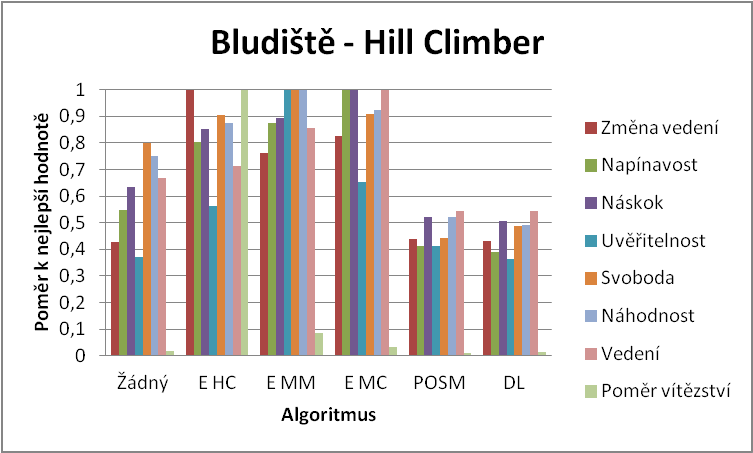
\includegraphics[width=0.75\textwidth]{ch5mazehc}
	\caption{Srovnání DDA alg. ve hře Bludiště s Hill Climber hráčem.}
	\label{fig-ch5mazehc}
\end{figure}

Z tabulky a především z grafu lze vyčíst, že algoritmy POSM a DL zaostávají nejen za ostatními DDA algoritmy, ale také za hrou, kde není použit žádný DDA mechanismus. Dopadají hůře i v metrikách napínavost a náskok, na kterých je testovali jejich autoři.

Při bližším zkoumání jsem zjistil, že důvodem pro špatné chování je absence přizpůsobování se metrice svoboda. Oba algoritmy příliš ořezávají možné tahy hráče na průměrných 7 tahů během hry. Bez použití DDA je průměrná hodnota svobody 12. Při nízké svobodě má hráč ve hře malé množství dveří, kterými by se vydal. Ve hře existuje málo větvení a naopak dlouhé chodby. Z tohoto důvodu se hráči rychle snižuje neprobádaný prostor - dlouhé chodby bez postranních dveří často odříznou část mapy od hráče. 

Oba algoritmy pracují pouze s hloubkou 1 a často se dostanou do situace, kdy už musí vytvořit chodbu k poslední bombě, přestože hráči zbývá ještě dostatek času. Případně nastane zcela opačná situace. Na mapě je více jak jedna bomba, tedy tyto algoritmy mohou bombu, ke které směřuje hráč, odříznout a udělat z ní falešnou, ale jelikož jsou ve hře především dlouhé nevětvené chodby, hráč se musí vrátit o velké množství kroků a vyprší mu čas.

\begin{table*}[b]\footnotesize
\vspace*{0mm}
\caption{{\label{tab-mazem}} Porovnání metrik zábavnosti u jednotlivých algoritmů ve hře Bludiště. }
\vspace*{0mm}
\label{shadowtable}
\begin{center}
\begin{tabular}{| l || r | r | r | r | r | r | r | r | r | r |}
\hline
Algoritmus & Počet kol	& Změna vedení & Napínavost & Náskok & Uvěřitelnost\\
\hline
\hline
Žádný & 93,127 & 8,217 & 343,6848421 & 239,851 & 81789,7937 \\ \hline  
E HC & 114,905 & 19,176 & 233,9169735 & 177,951 & 53868,86 \\ \hline
E MM & 113,32 & 14,64 & 214,5392914 & 169,935 & 30377,59274 \\ \hline
E MC & 105,494 & 15,829 & 187,5847573 & 151,923 & 46656,61097 \\ \hline
POSM & 99,902 & 8,394 & 455,7661817 & 290,602 & 73884,68107 \\ \hline
DL & 95,431 & 8,29 & 483,7274291 & 300,486 & 83988,2358 \\ \hline
\end{tabular}
\end{center}
\begin{center}
\begin{tabular}{| l || r | r | r | r | r | r | r | r | r |}
\hline
Algoritmus & Svoboda & Náhodnost & Vedení &	Rozptyl Vítězů \\
\hline
\hline
Žádný & 12,19857537 & 15,05552294 & 33,04804979 & 0,121 \\ \hline  
E HC & 13,79978394 & 12,92183276 & 31,00734155 & 0,002 \\ \hline
E MM & 15,26174269 & 11,29628595 & 25,74151376 & 0,024 \\ \hline
E MC & 13,84465841 & 12,22155687 & 22,05607333 & 0,065 \\ \hline
POSM & 6,76593984 & 21,72255666 & 40,54974306 & 0,176 \\ \hline
DL & 7,45030571 & 22,91638791 & 40,45994322 & 0,154 \\ \hline
\end{tabular}
\end{center}
\end{table*}

Algoritmy E-HC, E-MM a E-MC dopadly obdobně. Algoritmu E-HC se nejlépe dařilo v metrikách poměr vítězství a změna vedení, E-MM zvítězil v uvěřitelnosti, náhodnosti a svobodě, E-MC dopadl nejlépe v napínavosti, náskoku a ve vedení.

\subsection{Vzhled bludiště pro různé DDA algoritmy}

\section{Ludo}

\begin{figure}
  \centering
  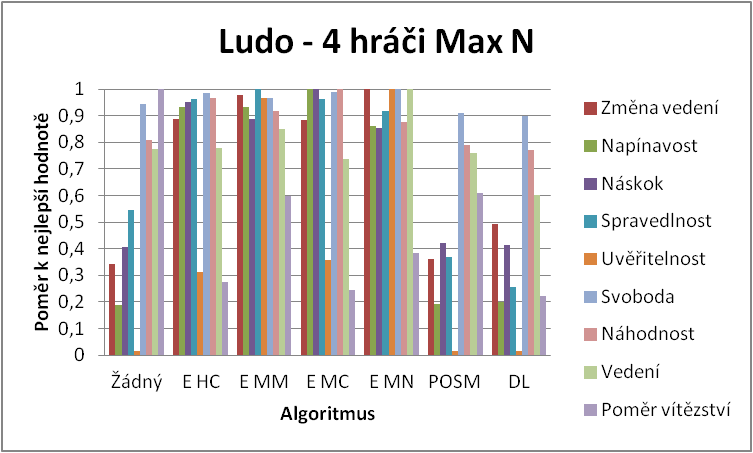
\includegraphics[width=0.75\textwidth]{ch5ludo4maxn}
	\caption{Srovnání DDA alg. ve hře Ludo se 4 Max N hráči. (úrovně 50, 100, 100, 100)}
	\label{fig-ch5ludo4maxn}
\end{figure}

\section{Ztracená města}

\begin{figure}
  \centering
  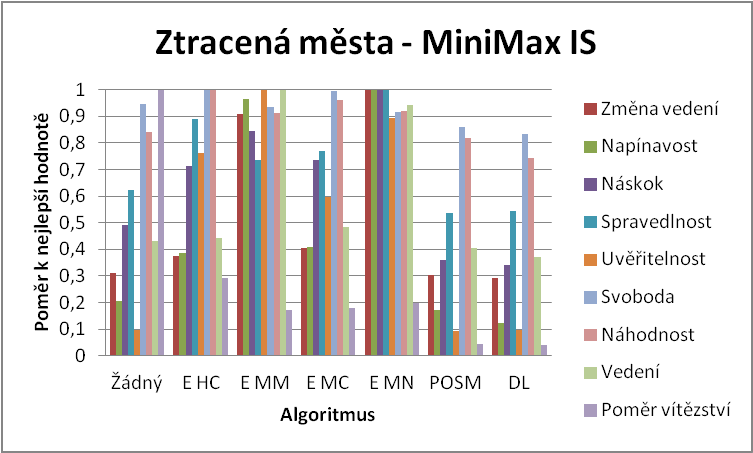
\includegraphics[width=0.75\textwidth]{ch5lcmm}
	\caption{Srovnání DDA alg. ve hře Ztracená Města s dvěma MiniMax IS hráči. (úrovně 50 a 100)}
	\label{fig-ch5lcmm}
\end{figure}

\section{Celkové srovnání}
\begin{figure}
  \centering
  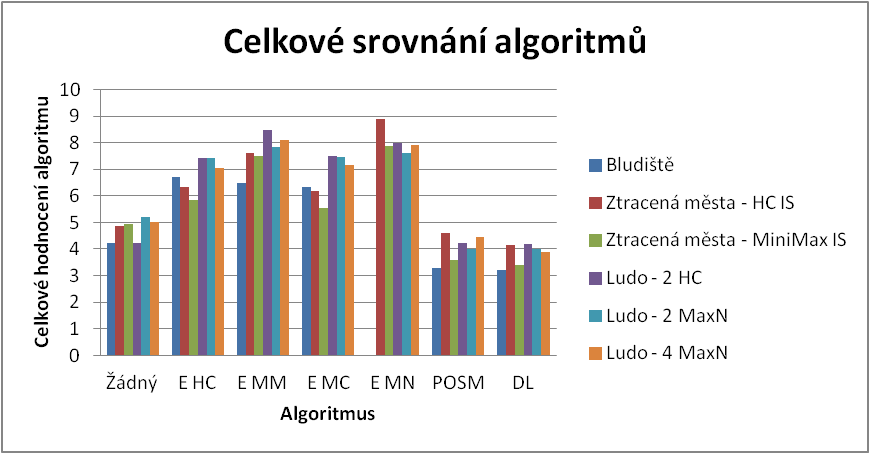
\includegraphics[width=0.80\textwidth]{ch5all}
	\caption{ Srovnání alg. DDA na základě všech experimentů a metrik. }
	\label{fig-ch5all}
\end{figure}

\begin{figure}
  \centering
  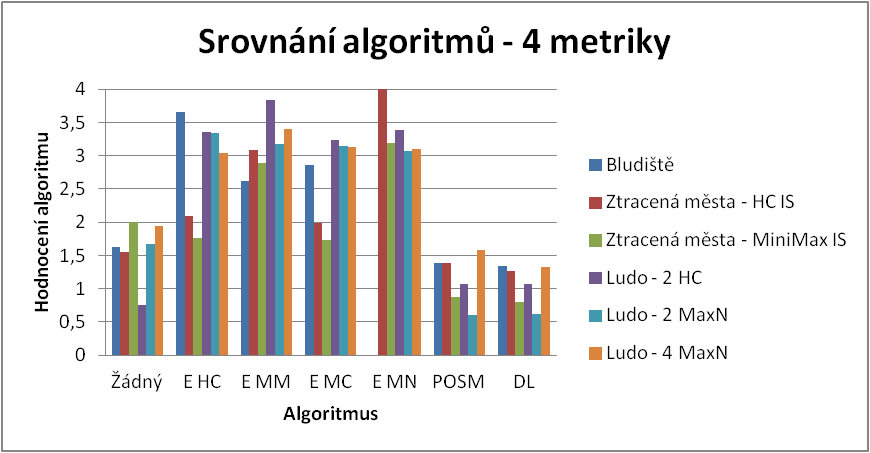
\includegraphics[width=0.80\textwidth]{ch5all4m}
	\caption{ Srovnání alg. DDA na základě všech experimentů a metrik Změna vedení, Napětí, Náskok a Poměr vítězů. }
	\label{fig-ch5all4m}
\end{figure}

\endinput
%%
%% End of file `ch01.tex'.
